\chapter{Conclusion}
\label{Chapter4}

\section{Bilan}
% Bilan : où j'en suis, ce qui a été réalisé, choix bon pas bon  1/2p, si + 1p faire chapitre "Discussion"
% Conclusion :résumer la réalisation 1/4p reprend souvent objectif (cet outil peut être très utile…..)
% Perspective : où on va a partir de la 1/4p -> peut inclure BIM/SIG

Il est maintenant temps de faire un bilan de l'état actuel du projet, d'analyser ce qui a bien été, les problèmes rencontrés et ce qui aurait pu être fait autrement.

Les analyses préliminaires ont pu être menées à bien, grâce à suffisament d'explications et de descriptions de cas réels données lors des séances avec Prof. Olivier Donzé. Il aurait été intéressant d'interroger d'autres personnes du domaine afin de confirmer, et éventuellement compléter, les besoins mentionnés en \ref{sec:requirements-analysis}.

Le bilan quant à la réalisation du prototype est, lui, plus mitigé. Utiliser des librairies ou des projets existants implique que l'on s'adapte aux technologies qu'ils emploient. 
En l'occurence, dans le cas présent, travailler avec la visionneuse choisie comme base (\textit{three-gltf-viewer}, \ref{sec:three-gltf-viewer}) s'est avérée plus difficile que prévu. 
D'une part, \textit{JavaScript} étant un langage interprété, les éventuels problèmes ne sont détectés qu'à l'exécution, ce qui a ralenti le flux de travail, en obligeant à répéter sans cesse certaines opérations pour s'assurer que tout fonctionne. 
D'autre part, l'essentiel du code de ce projet est condensé dans un seul fichier, plutôt que réparti en plusieurs de plus petite taille et traitant chacun d'une partie spécifique, ce qui ne facilite pas la navigation. 
Enfin, il utilise plusieurs librairies externes (\textit{NodeJS}, \textit{Electron},...), impliquant de connaître également ces technologies ou s'y former si l'on ne veut pas se retrouver bloqué lorsque l'on souhaite apporter des modifications.
De nombreux problèmes rencontrés ont ainsi ralenti le développement, expliquant pourquoi le prototype n'inclut pas autant de fonctionnalités que souhaitées.
Néanmoins, une petite démo fonctionnelle a pu être réalisée, ce qui n'aurait certainement pas été le cas en partant totalement de zéro.

D'un point de vue personnel, ce projet a été très enrichissant car il m'a permis de découvrir de nombreux aspects du domaine de l'urbanisme, et d'étudier de nombreuses technologies associées. J'aurais néanmoins apprécié pouvoir proposer un prototype plus complet.

\section{Travail réalisé}
Ce projet a mis en évidence l'intérêt que présente la réalisation d'une plateforme de modèles 3D destinée au domaine de l'urbanisme. Ses avantages sont principalement :

\begin{itemize}
    \item Faciliter les interactions entre les différents acteurs de la modélisation du paysage ainsi qu'avec la population, en proposant un point central, toujours accessible, où les échanges peuvent avoir lieu.
    \item Permettre une communication améliorée, plus précise, sur des parties précises d'un modèle, gâce aux annotations.
    \item Pouvoir être adaptée à d'autres besoins du secteur de la modélisation du paysage, actuels ou futurs, en ajoutant d'autres modules.
\end{itemize}

La faisabilité de conception de cet outil a été démontrée.\todo{phrase à virer ?}

La phase d'analyse a permis d'une part d'identifier les "briques" qui pourraient la composer, et d'autre part de proposer une architecture générale.

Pour chaque module, les technologies correspondantes ont été étudiées et des solutions, notamment basées sur des librairies ou projets déjà existants, ont été offertes. 
L'aspect libre (\textit{open-source}) a été privilégié lors des choix, afin de garantir des possibilités d'évolution et de collaboration autour du développement de l'outil. Aussi, assurer l'indépendance envers toutes technologies ou produits fermés offre de meilleures chances d'adoption et d'intégration d'un tel système.

L'ajout d'annotations liées à des parties spécifiques d'un modèle est ressorti comme étant une fonctionnalité-clé. 
En effet, cela apporte une réelle plus-value à la communication entre les différents acteurs de l'urbanisme autour du projet : il devient ainsi possible d'échanger aisément, de façon différée, à propos d'éléments précis du modèle. 
Sans la possibilité d'associer des remarques aux coordonnées qu'elles concernent, il peut être difficile de faire le lien seulement à partir de leur contenu.

Enfin, le prototype réalisé illustre succinctement le résultat de ce travail de recherche.

\section{Perspective}
Ce travail peut servir de guide pour la réalisation d'une version concrète d'une telle plateforme. Afin que celle-ci s'intègre au mieux parmi les processus existants, il serait bienvenu d'étudier comment cet outil pourrait être assimilié dans le \textit{BIM}.

Le \textit{BIM} (\textit{Building Information Modeling}), illustré par la figure \ref{fig:bim-process}, est un processus de collaboration et d'échange d'information entre toutes les disciplines impliquées dans un projet d'urbanisme. En utilisant les outils et méthodes appropriés, l'ensemble des ressouces (modèles, informations...) est accessible et manipulable par chacun, des architectes aux entrepreneurs, en passant par les ingénieurs du bâtiment ou encore les fournisseurs, créant un effet de synergie \cite{buildingsmart}.

\begin{figure}[h]
    \centering
    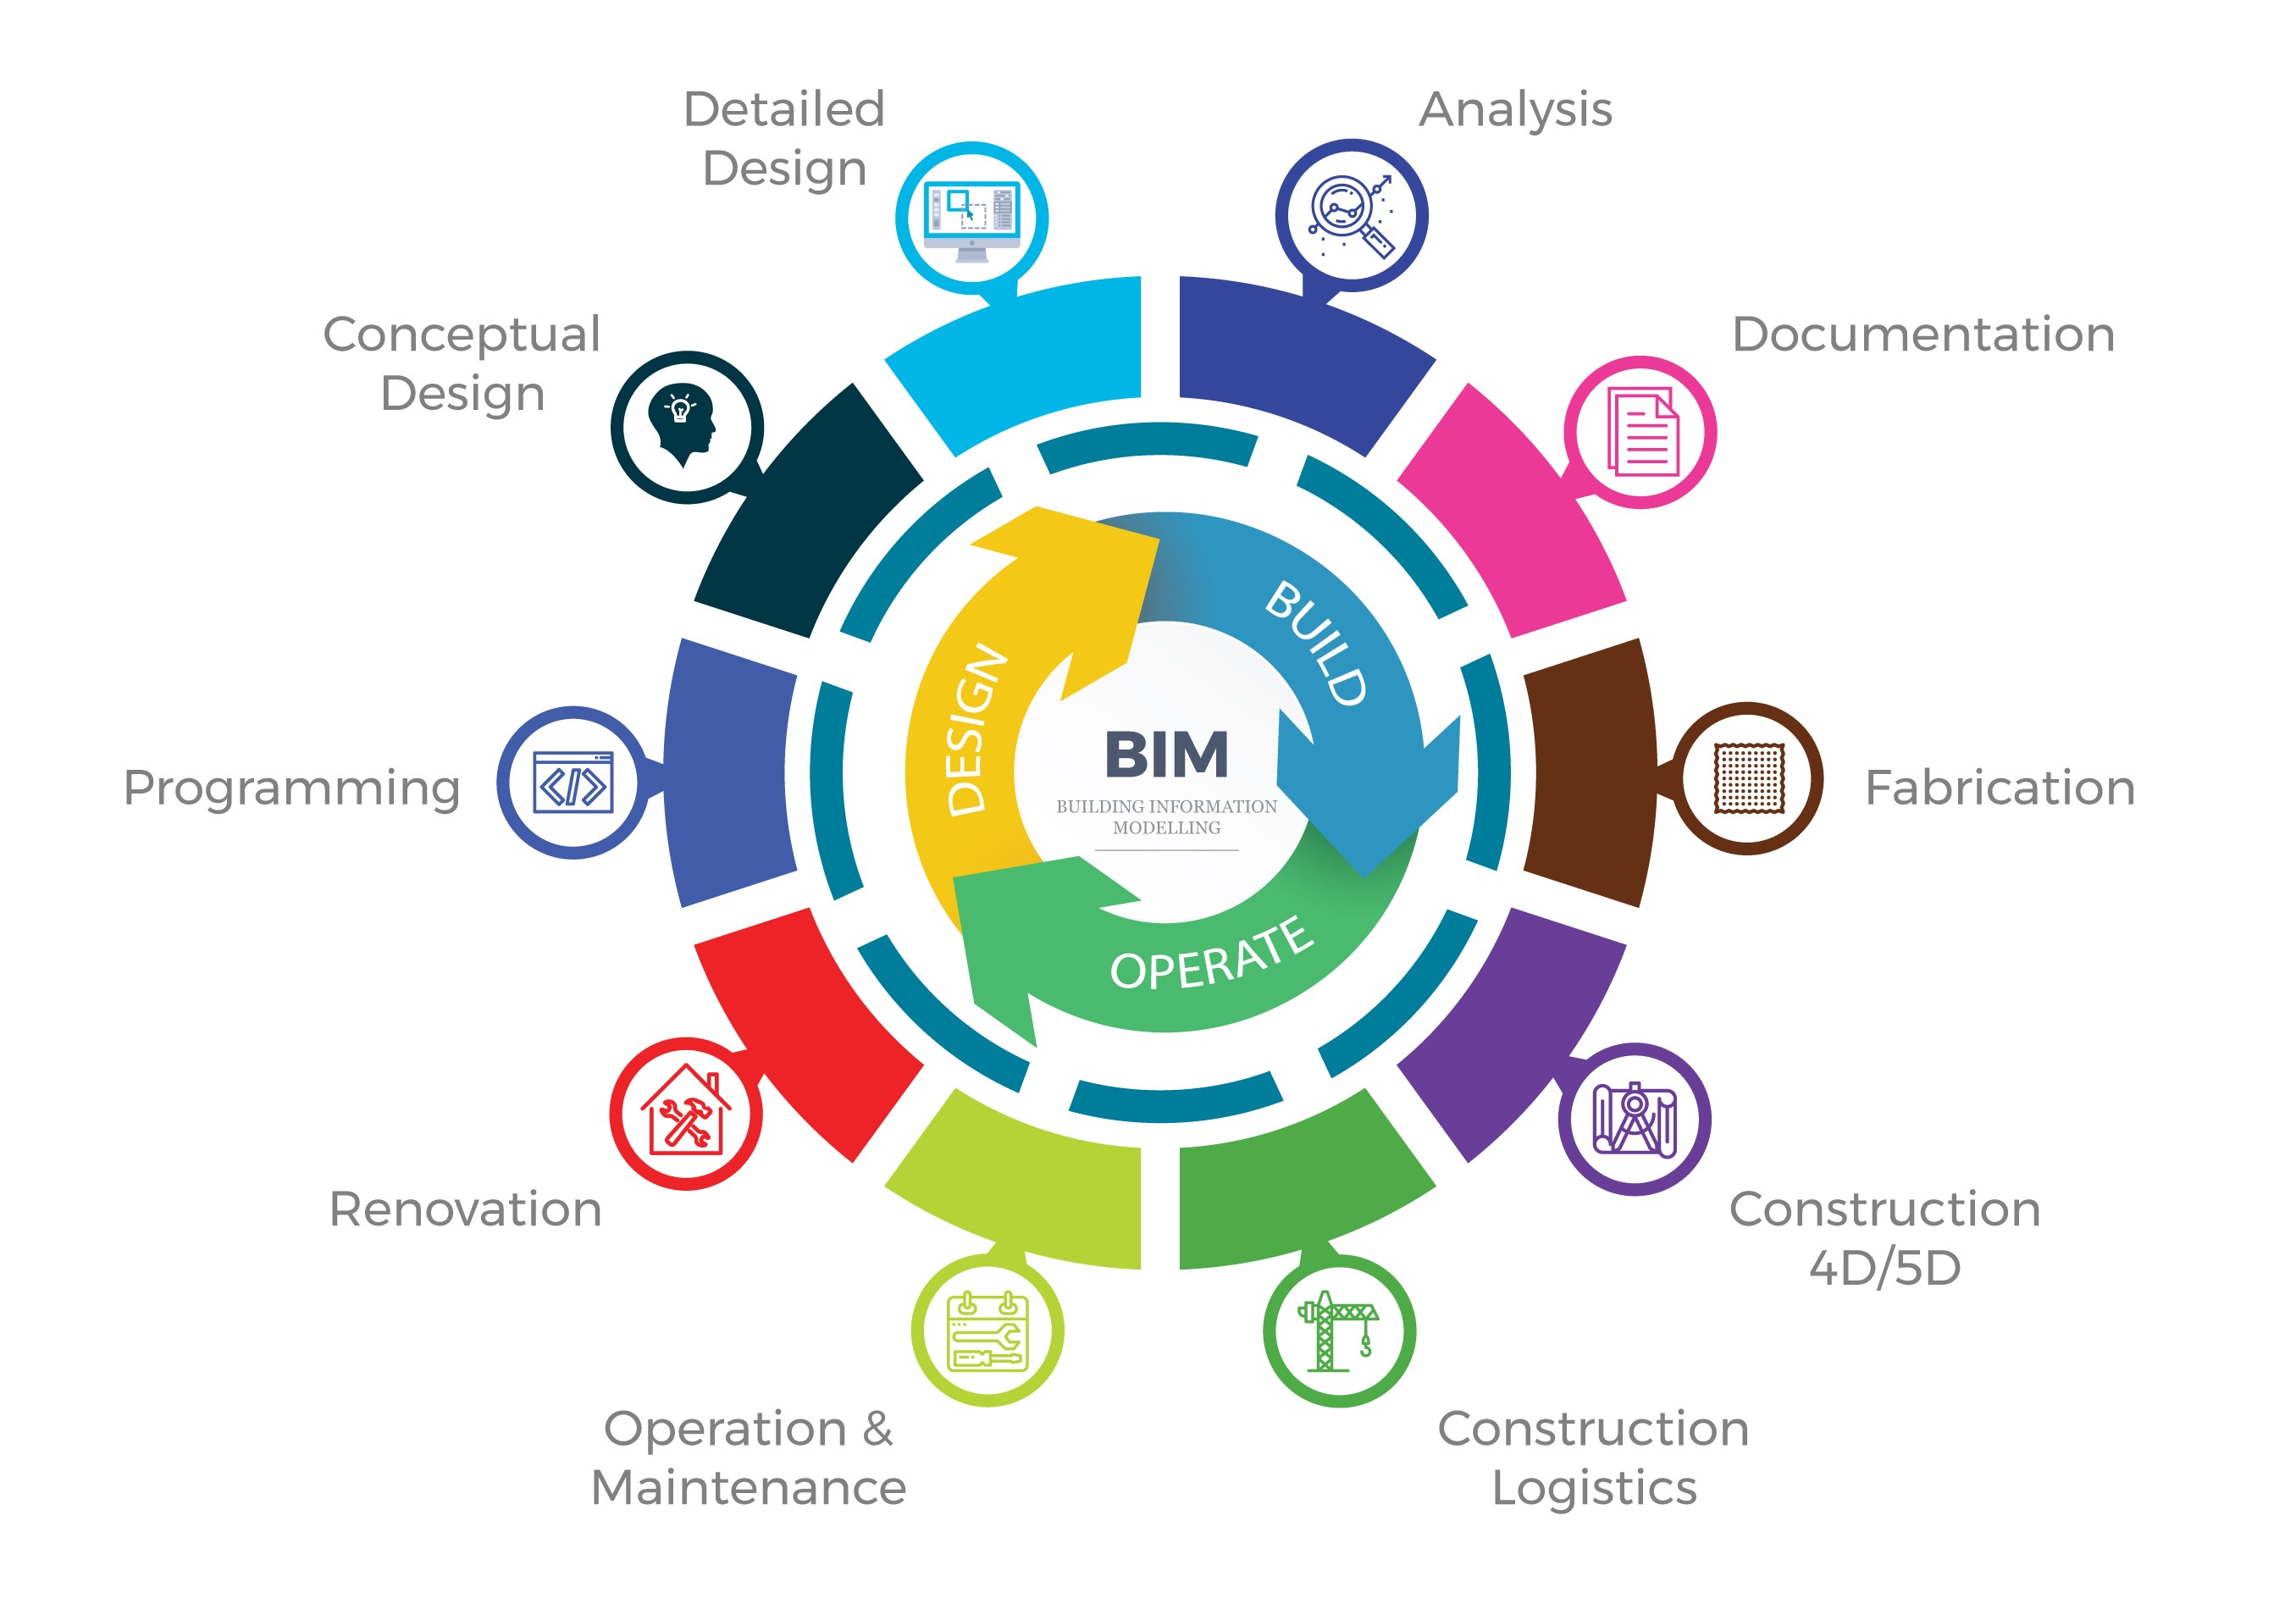
\includegraphics[width=0.7\linewidth]{Figures/bim-process.jpg}
    \caption{Processus BIM}
    \label{fig:bim-process}
\end{figure}

Il est également possible que les éditeurs actuels qui, s'adaptant progressivement au \textit{BIM} car y voyant là une nouvelle manne financière, ajoute un tel produit à leurs suites logiciels. Mais cela comportera alors les désavantages habituels, comme des licences exhorbitantes (se pose alors la question de "qui paie" pour que tous aient accès à l'outil) ou encore le fait d'être dépendant du bon vouloir de l'entreprise pour ajouter des fonctionnalités qui viendraient à manquer.  

Heureusement, l'existence de standards ouverts (tels que ceux proposés par le \textit{Khronos Group} (\ref{sec:khronos-group})), et la tendance à l'\textit{open-source} toujours croissante, laissent espérer qu'une solution libre fasse son apparition un jour.